%% 
\chapter{Optimizing Species-Specified Aerosol Emissions} \label{chap:}

\section{Introduction}

 In this chapter, we present a new attempt for the top-down estimate 
 of aerosol emissions through integration of the satellite observation 
 of reflectance and GEOS-Chem Adjoint model. 
 The technique is applied to improve estimates of mineral dust 
 and anthropogenic \ce{SO2}, \ce{NH3}, \ce{NOx}, \ce{BC} and \ce{OC} 
 emissions over China for April 2008, during which ground-based 
 PM\textsubscript{10} (particulate matter with aerodynamic diameter of 
 10 $\mu$m or less) data is available from a joint China-U.S. 
 dust field experiment [Huang et al., 2010]. 
 This paper differs from the past work in that: 
 (i) satellite reflectance (in essence radiance) is used 
 to constrain the emission estimates of aerosol particle and precursors, 
 which eliminates the discrepancy of aerosol optical properties 
 between model simulated and satellite retrieved AOD; 
 (ii) we use a suite of aerosol and gas measurements 
 from satellite sensors and ground-based instruments 
 to independently evaluate our results, and test our hypothesis 
 that temporal variation of AOD at different locations, 
 as characterized by satellite observations, can be a strong constraint 
 for species-specific source estimates if they are combined with 
 the model-based knowledge of the dominant aerosol sources 
 and the source-receptor relationship at corresponding locations; 
 and (iii) combination of (i) and (ii) will provide the basis and 
 a necessary step forward for future research to simultaneously 
 use both gas and AOD measurements to constrain speciated aerosol emissions. 

 We describe the top-down inversion scheme and its key components 
 (i.e., GEOS-Chem forward model and its adjoint, and observational constraints) 
 in Section 2. The top-down constraints on aerosol emissions over China 
 for the period of April 2008 are presented in Section 3, 
 and evaluated in Section 4. Interpretation and 
 implications of the results are discussed in Section 5, 
 and Section 6 summaries this study. [needs updates!!!!]

 \begin{figure}[h]
  \centering
  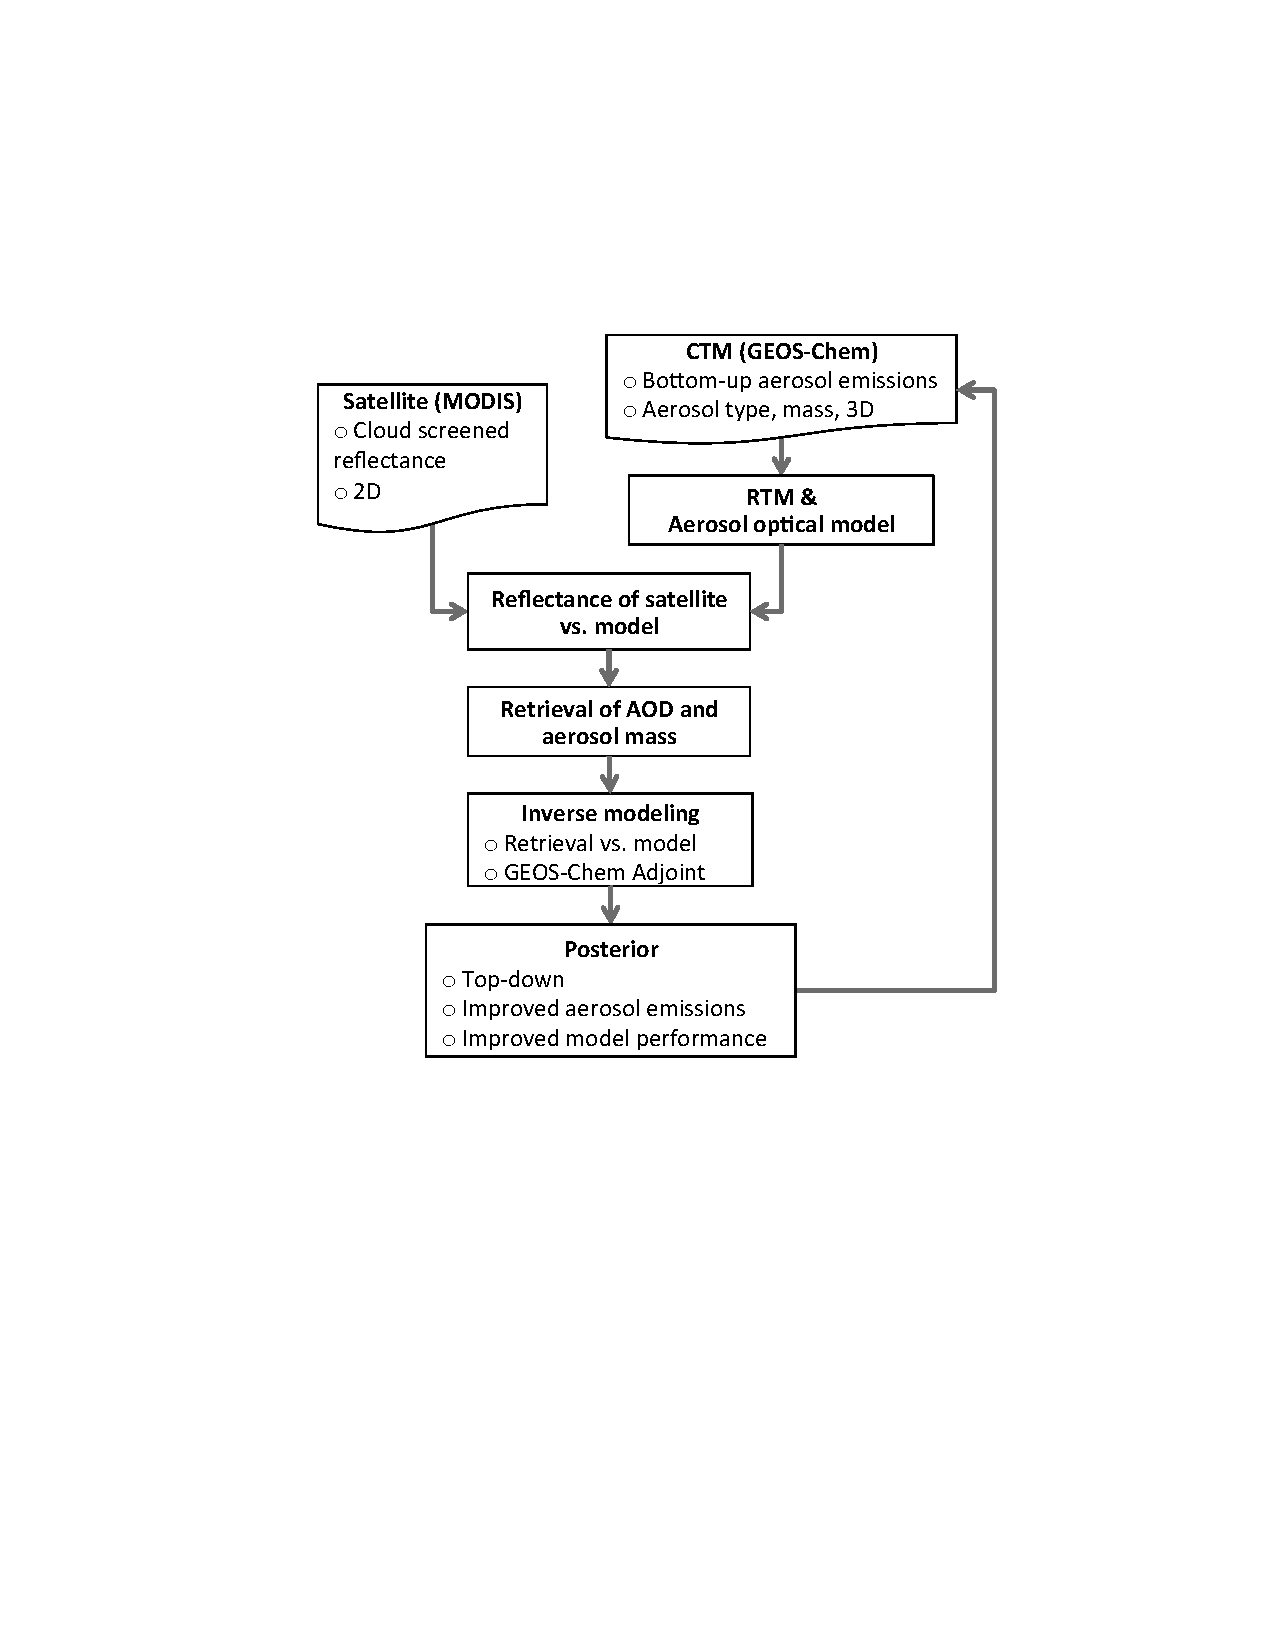
\includegraphics[width={0.7\textwidth}]{figures/a1.pdf}
  \caption{Flowchart of the proposed top-down inversion framework.}
  \label{fig:flowchat}
 \end{figure}

 As shown in Figure \ref{fig:flowchat}, the top-down inversion approach in this study 
 integrates the MODIS radiance/reflectance with the GEOS-Chem (section 2.1) 
 and its adjoint model (section 2.2) to optimize aerosol emissions. 
 First, similar to Wang et al. [2010], we retrieve the atmospheric 
 aerosol mass and AOD through fitting the calculated radiance based on 
 GEOS-Chem aerosol composition and single optical properties to the MODIS 
 cloud-free radiances (section 2.3). Second, the retrieved AOD 
 (hereafter retrieved MODIS AOD) from the first step is used as 
 an observational constraint to optimize the aerosol emissions 
 by inverting the GEOS-Chem chemical transport model (section 2.4). 
 The approach aims to improve aerosol emission estimates that ultimately 
 will yield better agreement between model simulated and satellite-observed 
 reflectances.  Since the aerosol single scattering properties are 
 exactly the same between the retrieval algorithm and GEOS-Chem 
 (as done in the first step), the top-down inversion scheme essentially 
 uses the MODIS radiances (in the form of retrieved AOD) to scale the 
 GEOS-Chem aerosol mass, which in turn are used to optimally adjust 
 the aerosol emissions. The approach here is first demonstrated through 
 a pseudo-observation experiment (Section 2.5) before it is applied 
 to real observations (Section 3).

\section{Constraints from Satellite Radiances}

\section{Selection of Emissions for Optimization and Sensitivity Tests}

 \begin{figure}[h]
  \centering
  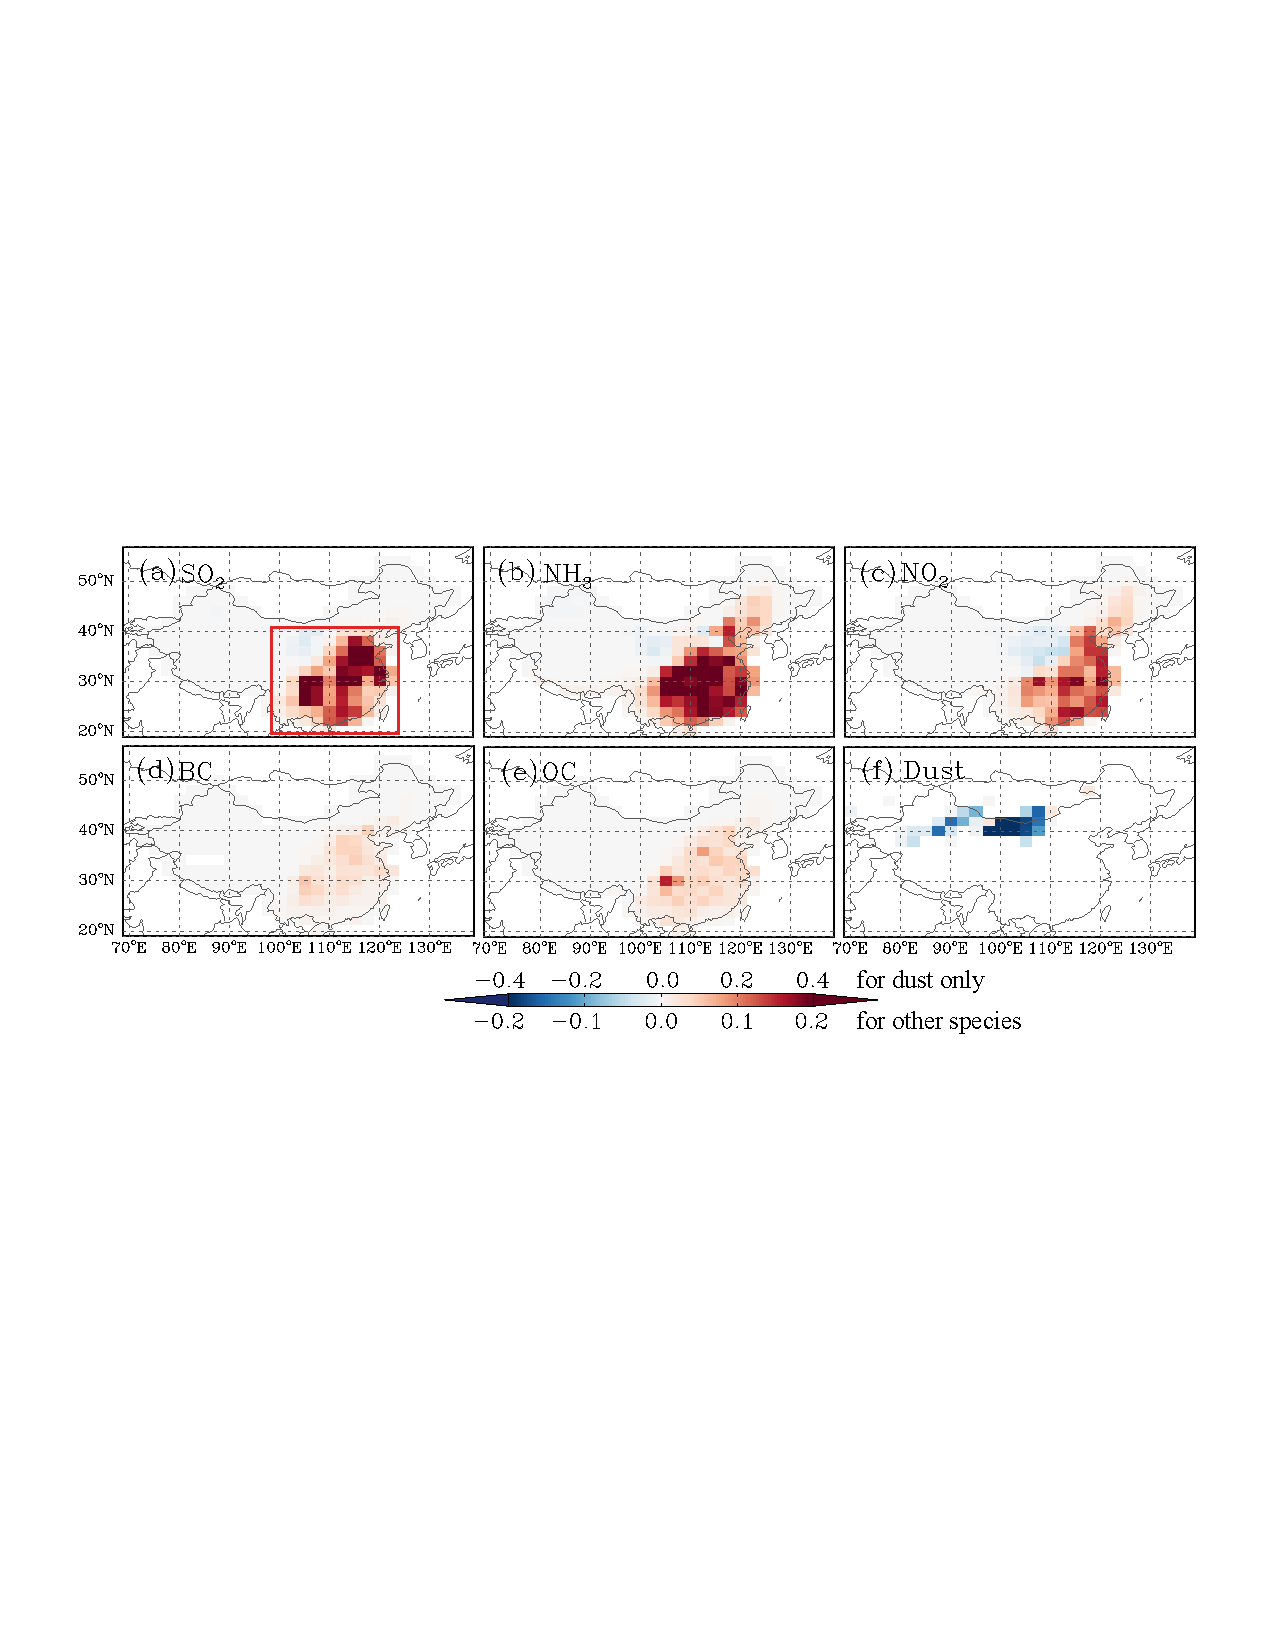
\includegraphics[width={0.9\textwidth}]{figures/a2.pdf}
  \caption{Relative changes in posterior aerosol emissions from \textit{a priori} 
   in the pseudo-observation experiment. 
   Six panels are respectively for anthropogenic emissions of \ce{SO2}, \ce{NH3}, 
   \ce{NOx}, BC, and OC, and mineral dust from both natural and anthropogenic sources. 
   The red box in panel (a) indicates the region where AOD observations are selected. }
  \label{fig:pseudo1}
 \end{figure}

\section{Inversion Results}

 \begin{figure}[h]
  \centering
  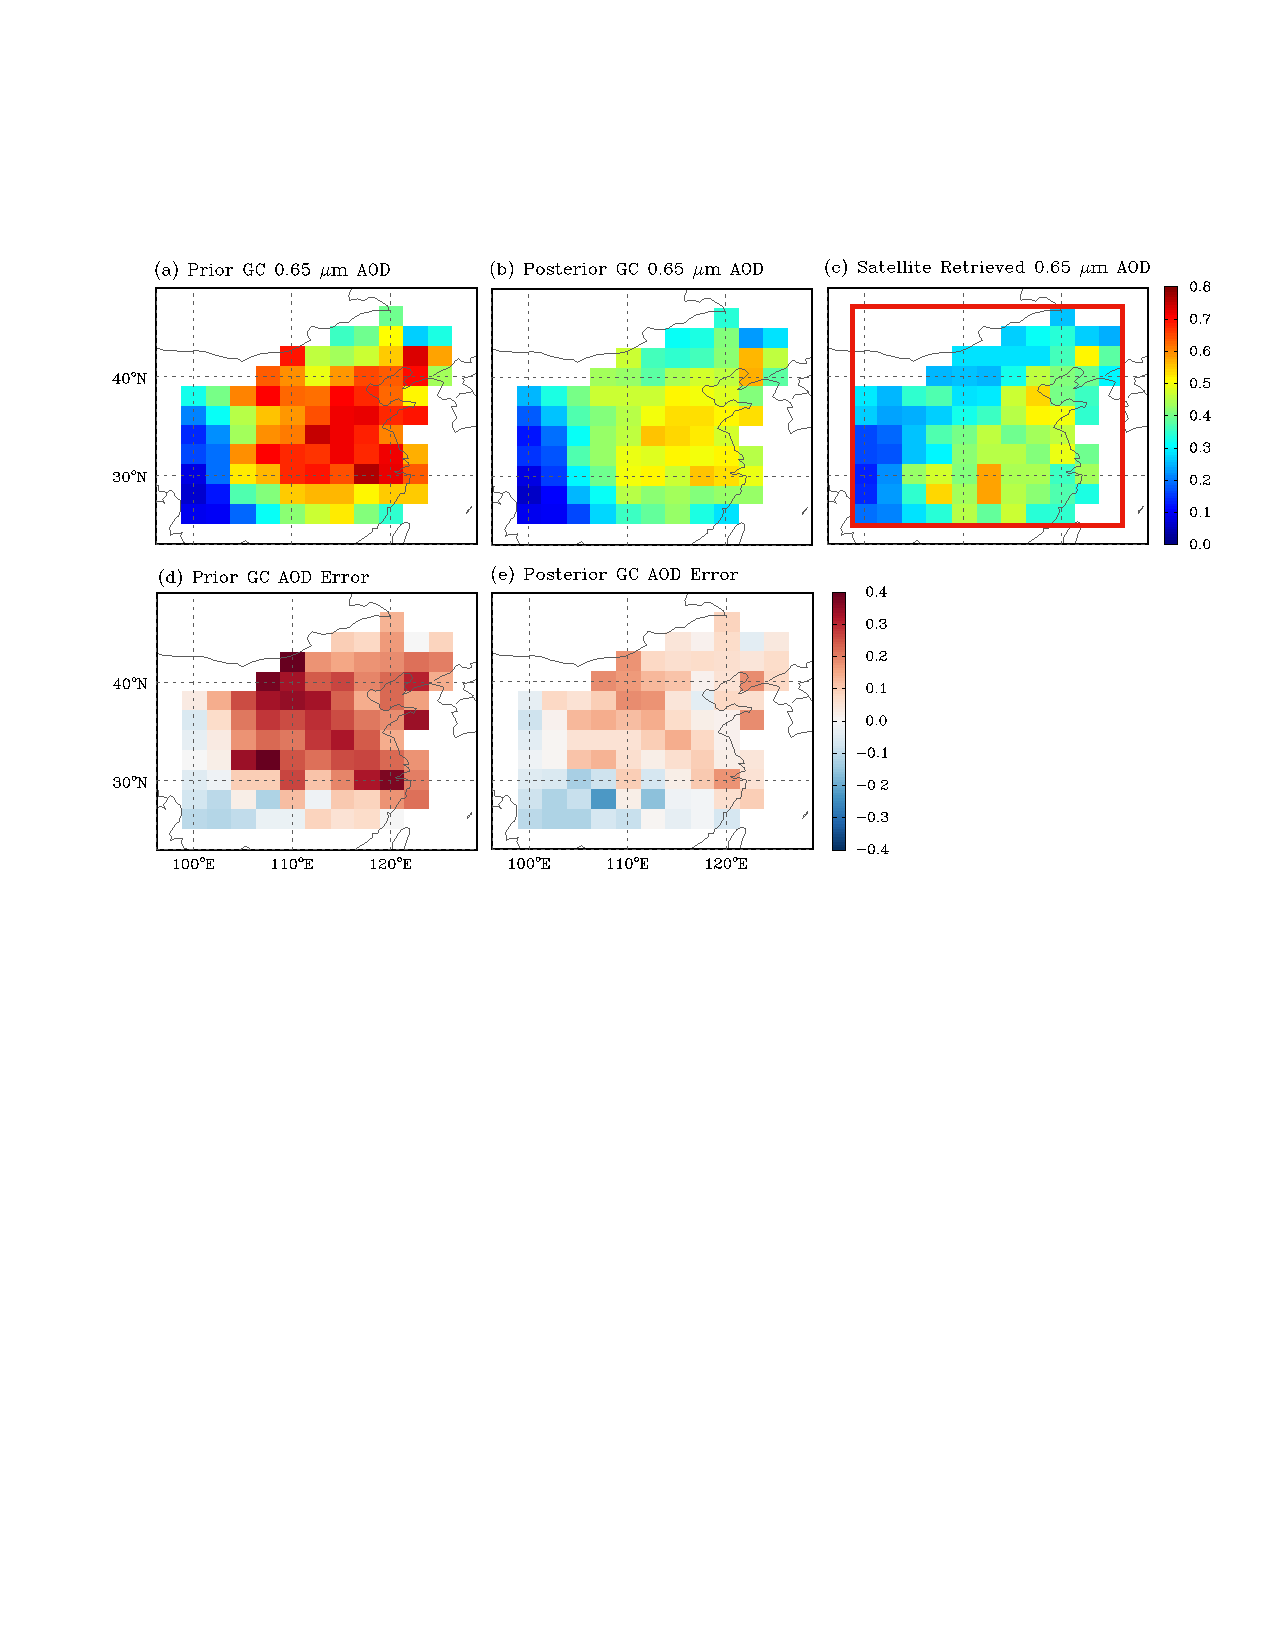
\includegraphics[width={0.9\textwidth}]{figures/a3.pdf}
  \caption{Comparison of the prior (a) and posterior (b) GEOS-Chem (GC) simulation 
 of 0.65 $\mu$m AOD with the AOD at the same wavelength retrieved from 
 MODIS reflectance using GEOS-Chem aerosol optical properties (c) averaged 
 for the period of April 2008. Satellite retrievals with 10 km by 10 km at nadir 
 are aggregated to GEOS-Chem grid cells; and the model AOD are sampled coincidentally 
 with those retrievals. Panel (d) and (e) respectively show the difference of 
 prior and posterior simulated from the satellite retrieved AODs. 
 The red box in panel (c) indicates the region where AOD observations are selected.}
  \label{fig:aods1}
 \end{figure}


 %% Figures of the daily variations in the AOD and dust emission
 \begin{figure}[t]
  \centering
  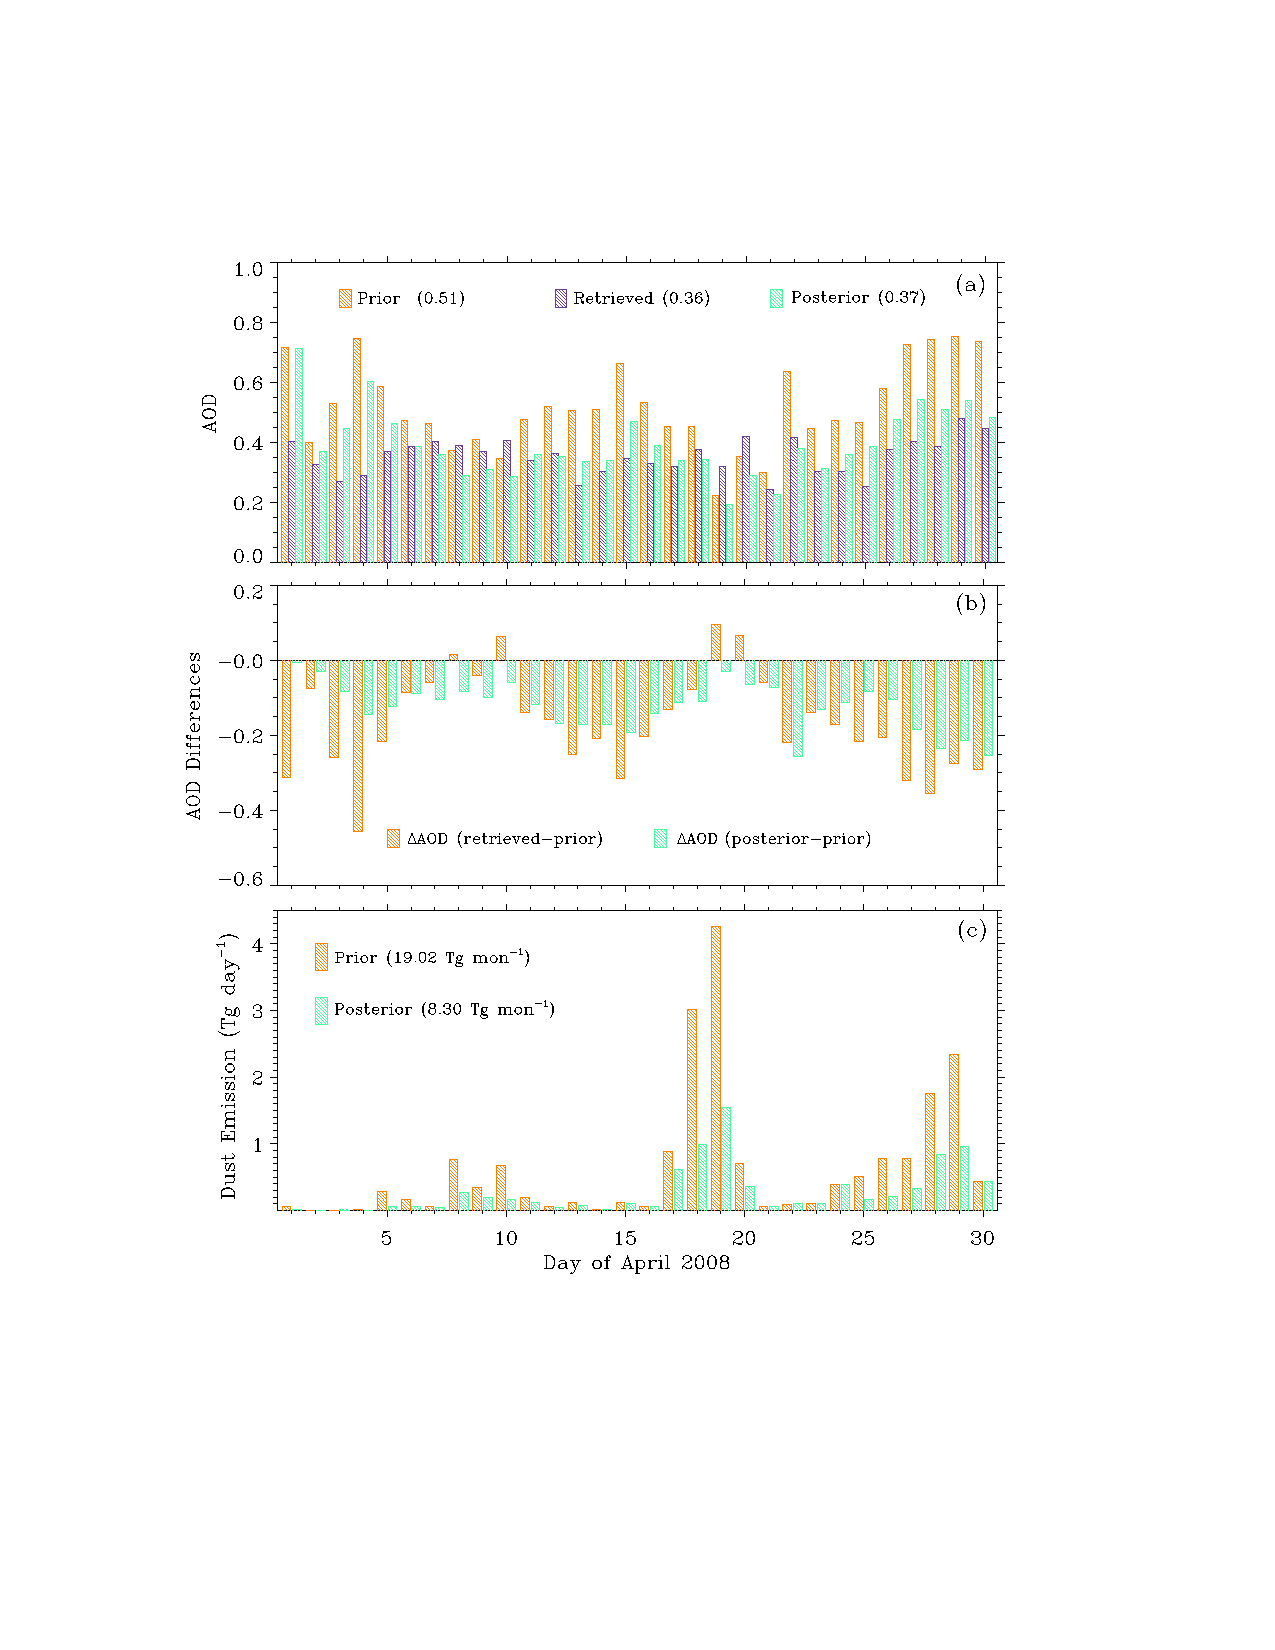
\includegraphics[width={0.75\textwidth}]{figures/a4.pdf}
  \caption{(a) Time series of the spatially averaged daily MODIS AOD retrievals (purple) for April 2008 over the Eastern China, compared by the prior (orange) and posterior (green) spatial averaged daily GEOS-Chem AOD that are sampled in the MODIS AOD tempo-spatial space. (b) Time series of the expected daily AOD adjustments (orange) that are the differences between MODIS AOD and the prior GEOS-Chem AOD and their real adjustments (green) that are the differences of posterior from prior GEOS-Chem AOD. (c) Time series of the prior (orange) and posterior (green) daily dust emissions over China for April 2008.}
  \label{fig:dailyaod}
 \end{figure}



 %% Figures of the optimized ems
 \begin{figure}[t]
  \centering
  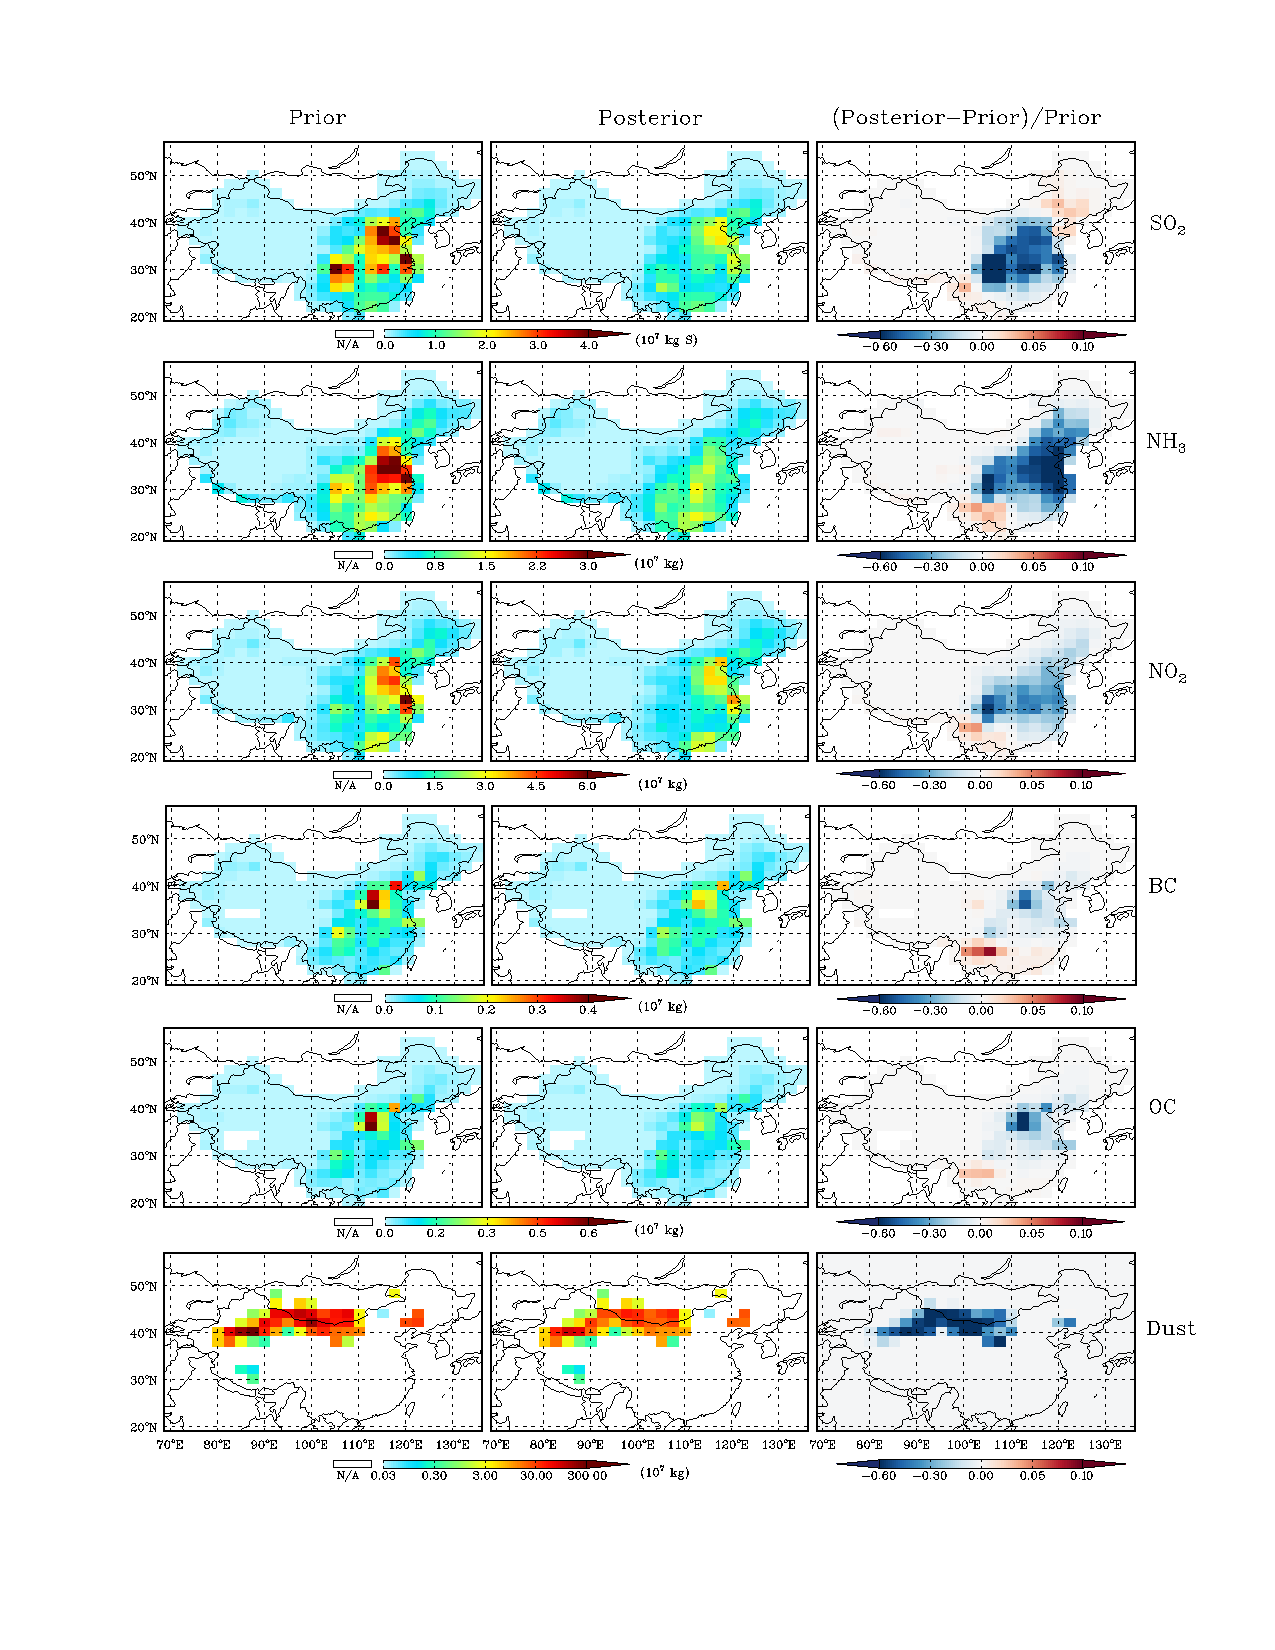
\includegraphics[width={0.90\textwidth}]{figures/a5.pdf}
  \caption{The prior (or bottom-up based, left column), optimized (or top-down constrained, middle column) aerosol emissions over China for the period of April 2008, and their relative differences (right column). Six rows from top to bottom are respectively for anthropogenic emissions of \ce{SO2}, \ce{NH3}, ce{NOx}, BC, and OC, and mineral dust from both natural and anthropogenic sources. }
  \label{fig:ems1}
 \end{figure}



\section{Results Evaluations} 

 %% Validation vs AEORNET
 \begin{figure}[b]
  \centering
  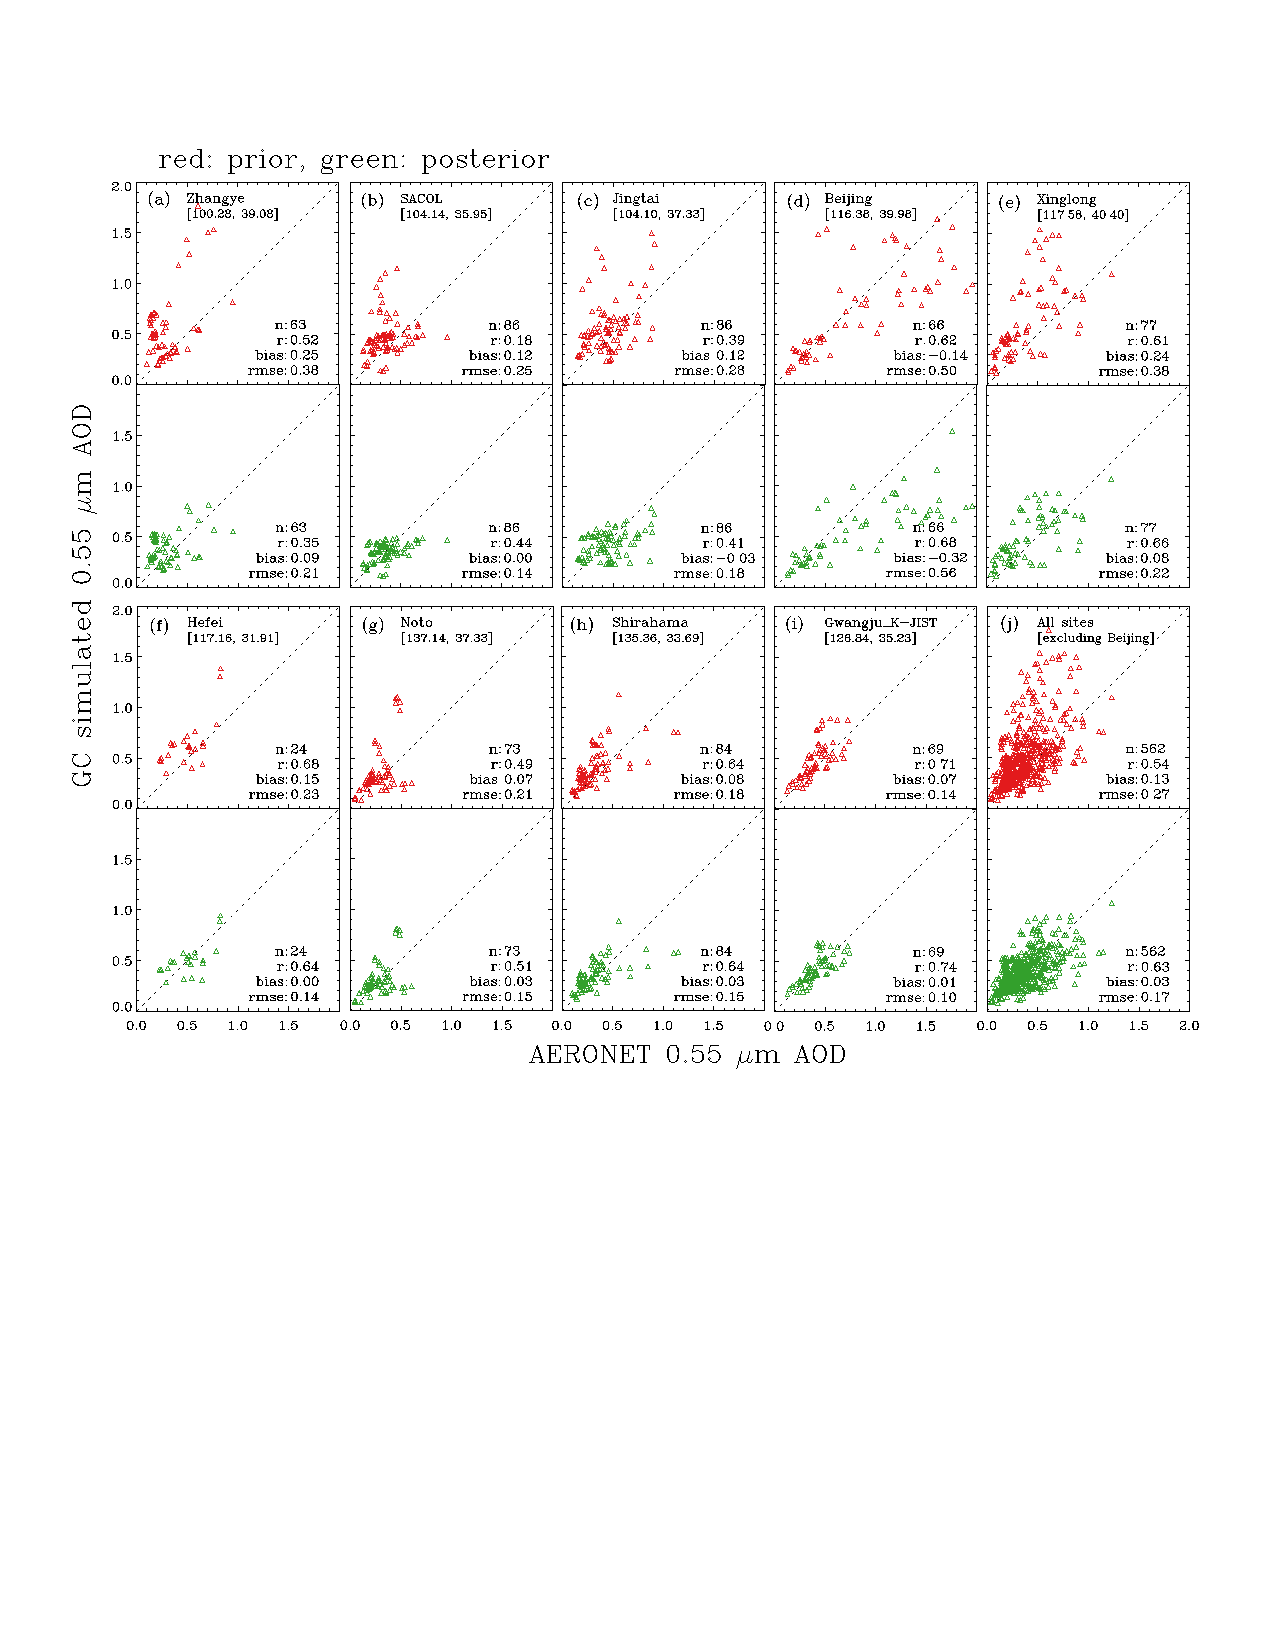
\includegraphics[width={0.99\textwidth}]{figures/a6.pdf}  
  \caption{(a – i) Scatterplots of GEOS-Chem AOD versus AERONET AOD at 0.55 $\mu$m prior (red scatters) and posterior (green scatters) to the aerosol emission optimization over nine stations. AERONET AODs are 3-hour averages following the GEOS-Chem output frequency. (j) The overall comparison for eight AERONET sites excluding Beijing. Also shown are the number of valid sampled pairs (n), correlation coefficients (R), bias, and root-mean-square-error (rmse).}
  \label{fig:aeronet1}
 \end{figure}


 %% Validation against MISR
 \begin{figure}[h]
  \centering
  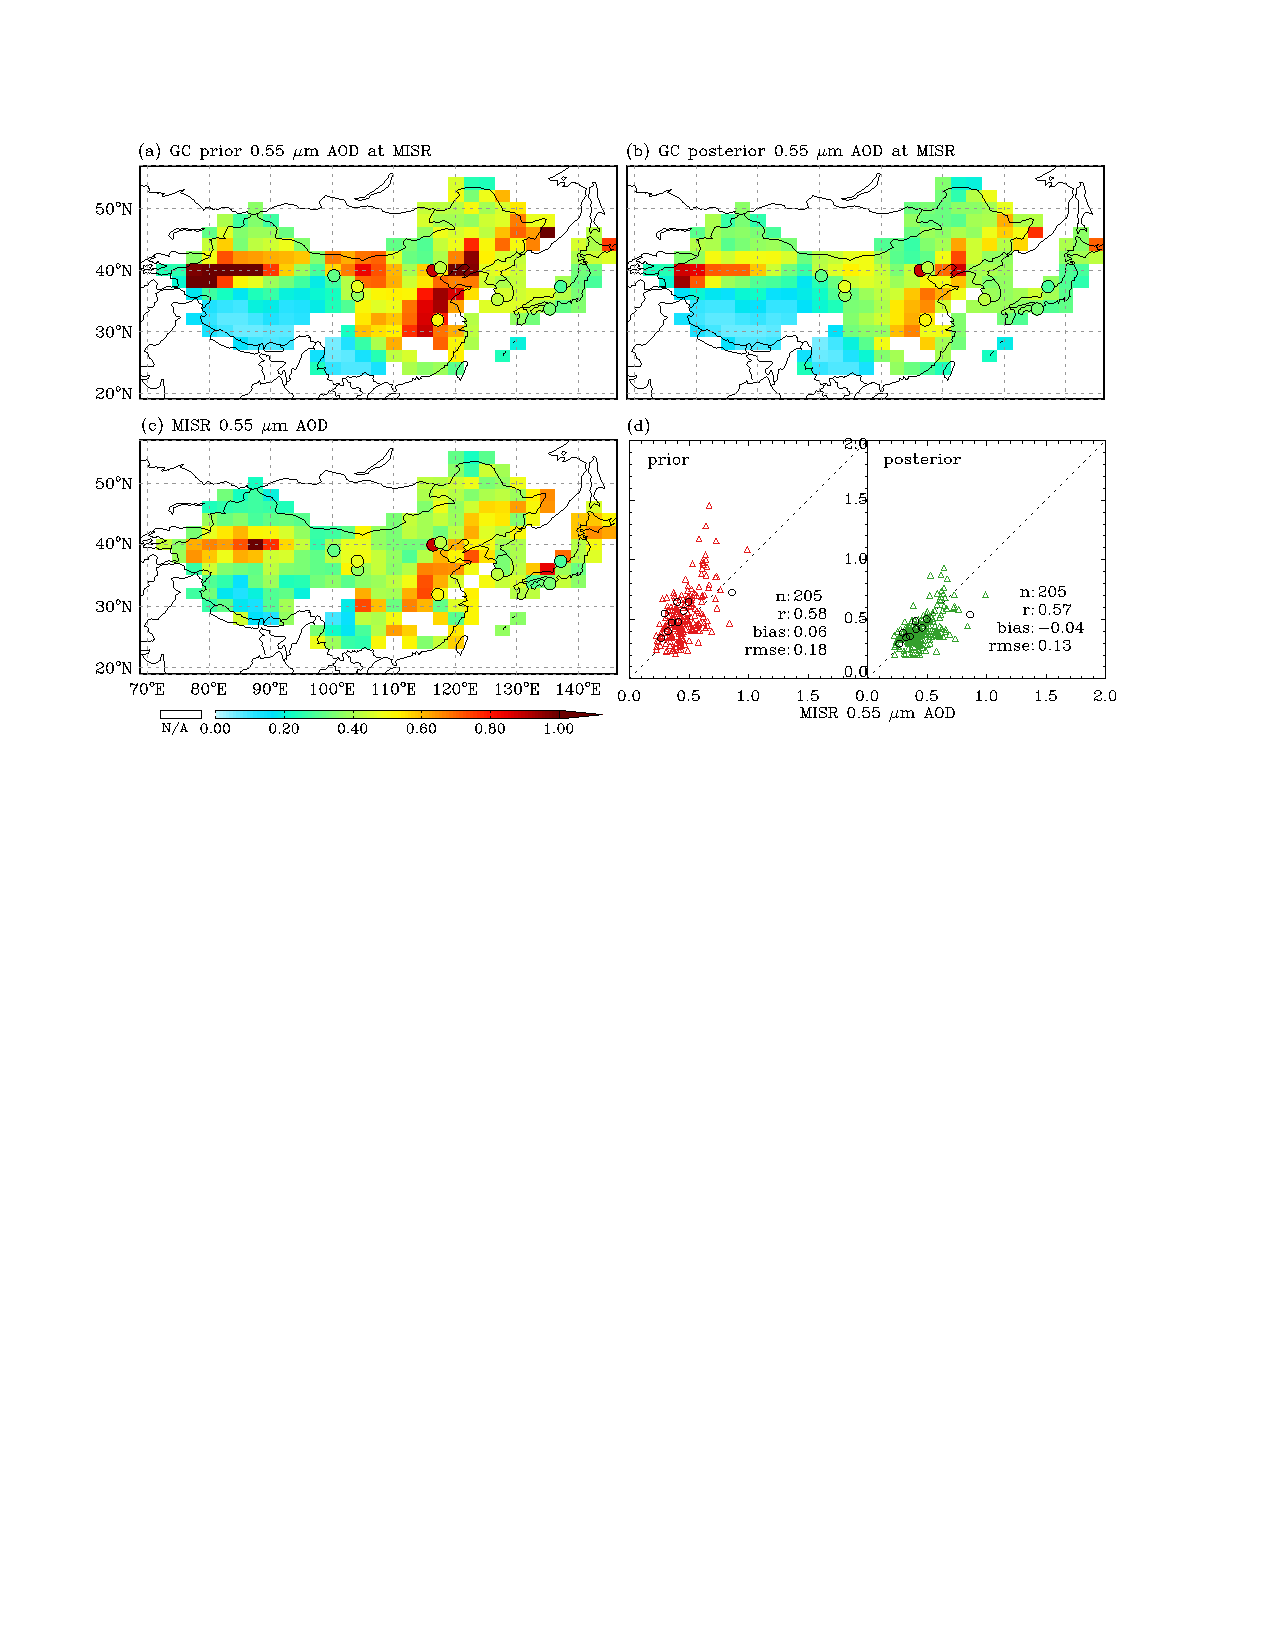
\includegraphics[width={0.9\textwidth}]{figures/a7.pdf}  
  \caption{Comparison of the prior and posterior GEOS-Chem simulation of 0.55 $\mu$m AOD with the level 3 MISR 0.55 $\mu$m AOD for the period April 2008. (a) The prior GEOS-Chem 0.55 $\mu$ AOD that are sampled coincidentally with MISR AODs for the period of April 2008. Also overlaid circles are the monthly AOD averages at 0.55 $\mu$m observed from the nine AEORNET sites shown in Figure \ref{fig:aeronet1}. (b) Same as (a) but for the monthly average of posterior GEOS-Chem AOD. (c) Monthly average of the Level 3 daily MISR 0.55 $\mu$m AOD.  (d) Scatter plot the GEOS-Chem AOD versus the MISR AOD before (red scatters) and after optimization (green scatters), in which each point indicates an AOD pair over a model grid cell with value over 0.2. Also shown are the statistics including number of sampled pairs (n), correlation coefficient (R), bias and root-mean-square-error (rmse). Comparisons of the monthly GEOS-Chem AOD versus AERONET AOD are also included as the black circles; each circle indicates an AOD pair over an individual site.}
  \label{fig:misr1}
 \end{figure}

 %% Validation against OMI SO2
 \begin{figure}[h]
  \centering
  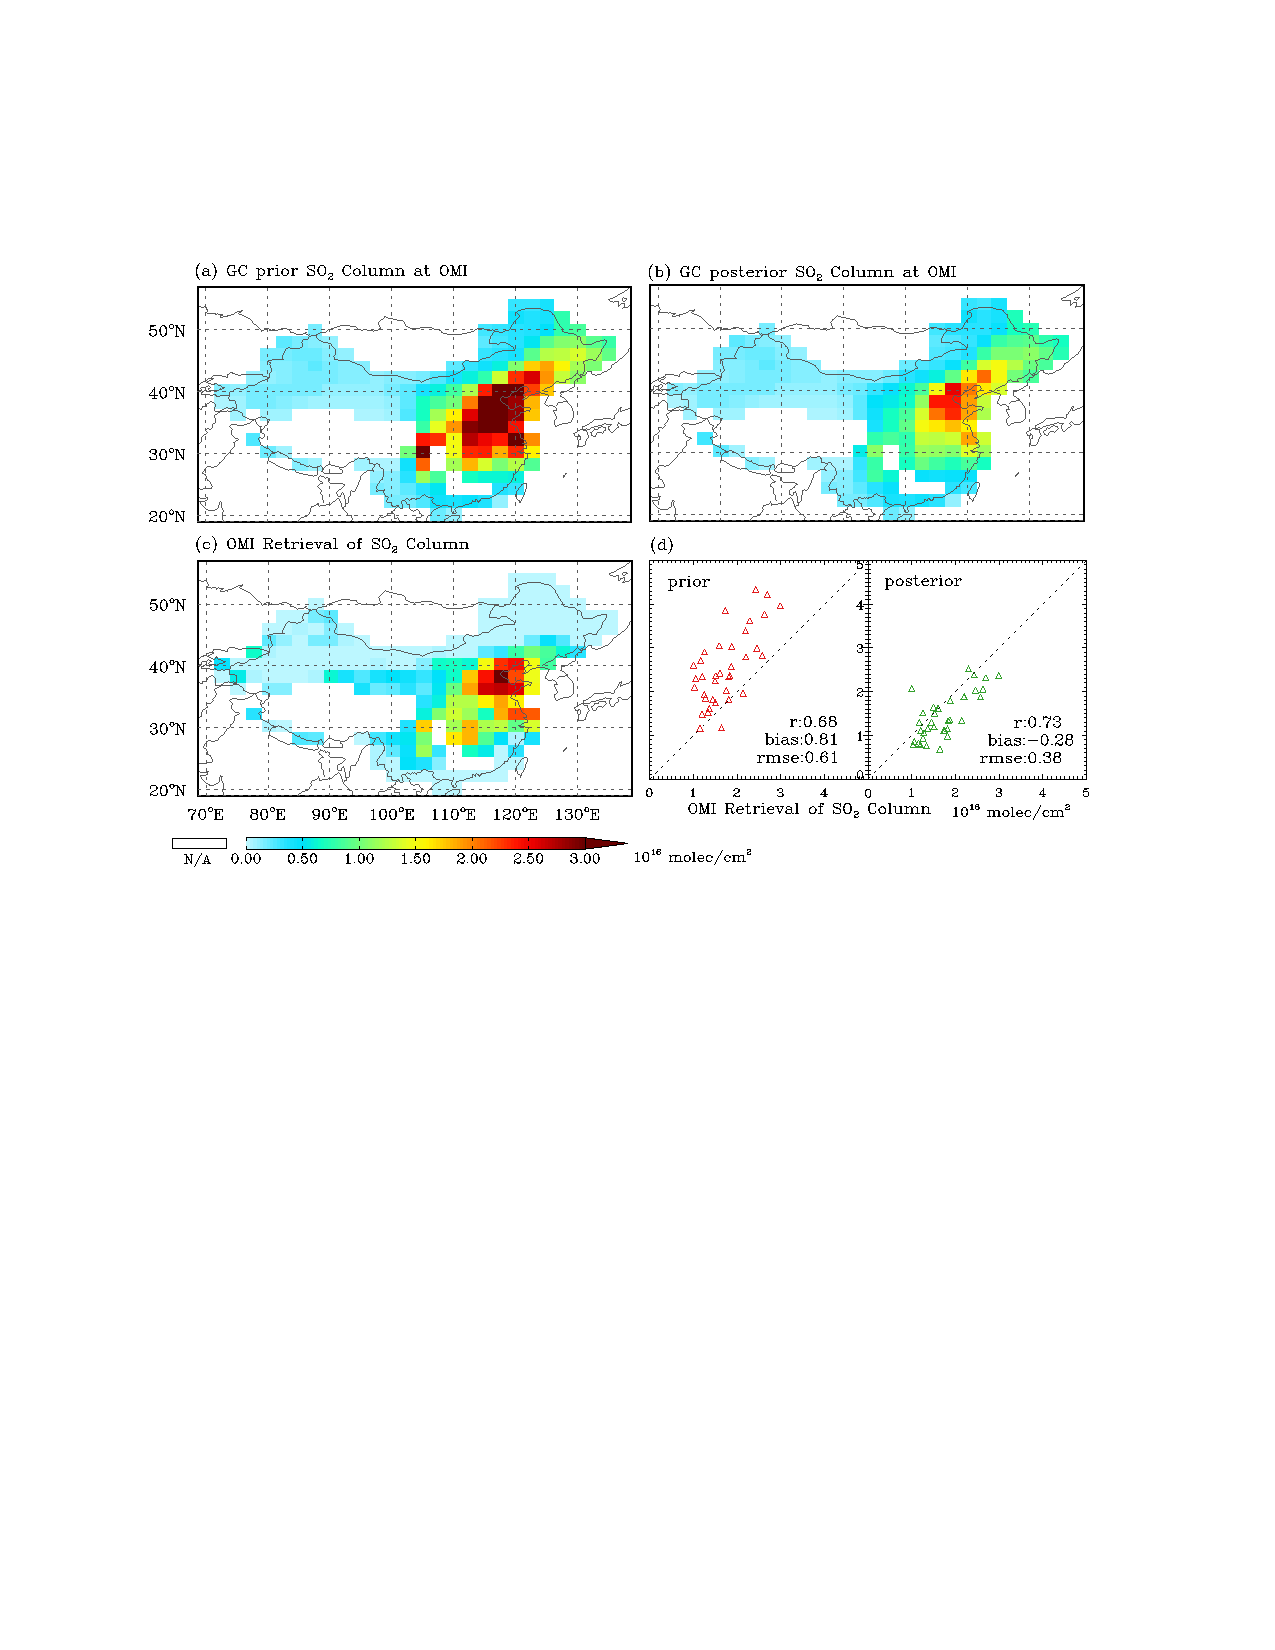
\includegraphics[width={0.9\textwidth}]{figures/a8.pdf}    
  \caption{Same as figure \ref{fig:misr1} but for comparison of the GEOS-Chem \ce{SO2} simulation with OMI column \ce{SO2} retrievals for the period of April 2008. The OMI planetary boundary layer (PBL) column \ce{SO2} from the Level 3 daily products with 0.25$^{\circ}$ by 0.25$^{\circ}$ resolutions are aggregated into GEOS-Chem grid cells.}
  \label{fig:omso2}
 \end{figure}

 %% Validation against OMI NO2
 \begin{figure}[h]
  \centering
  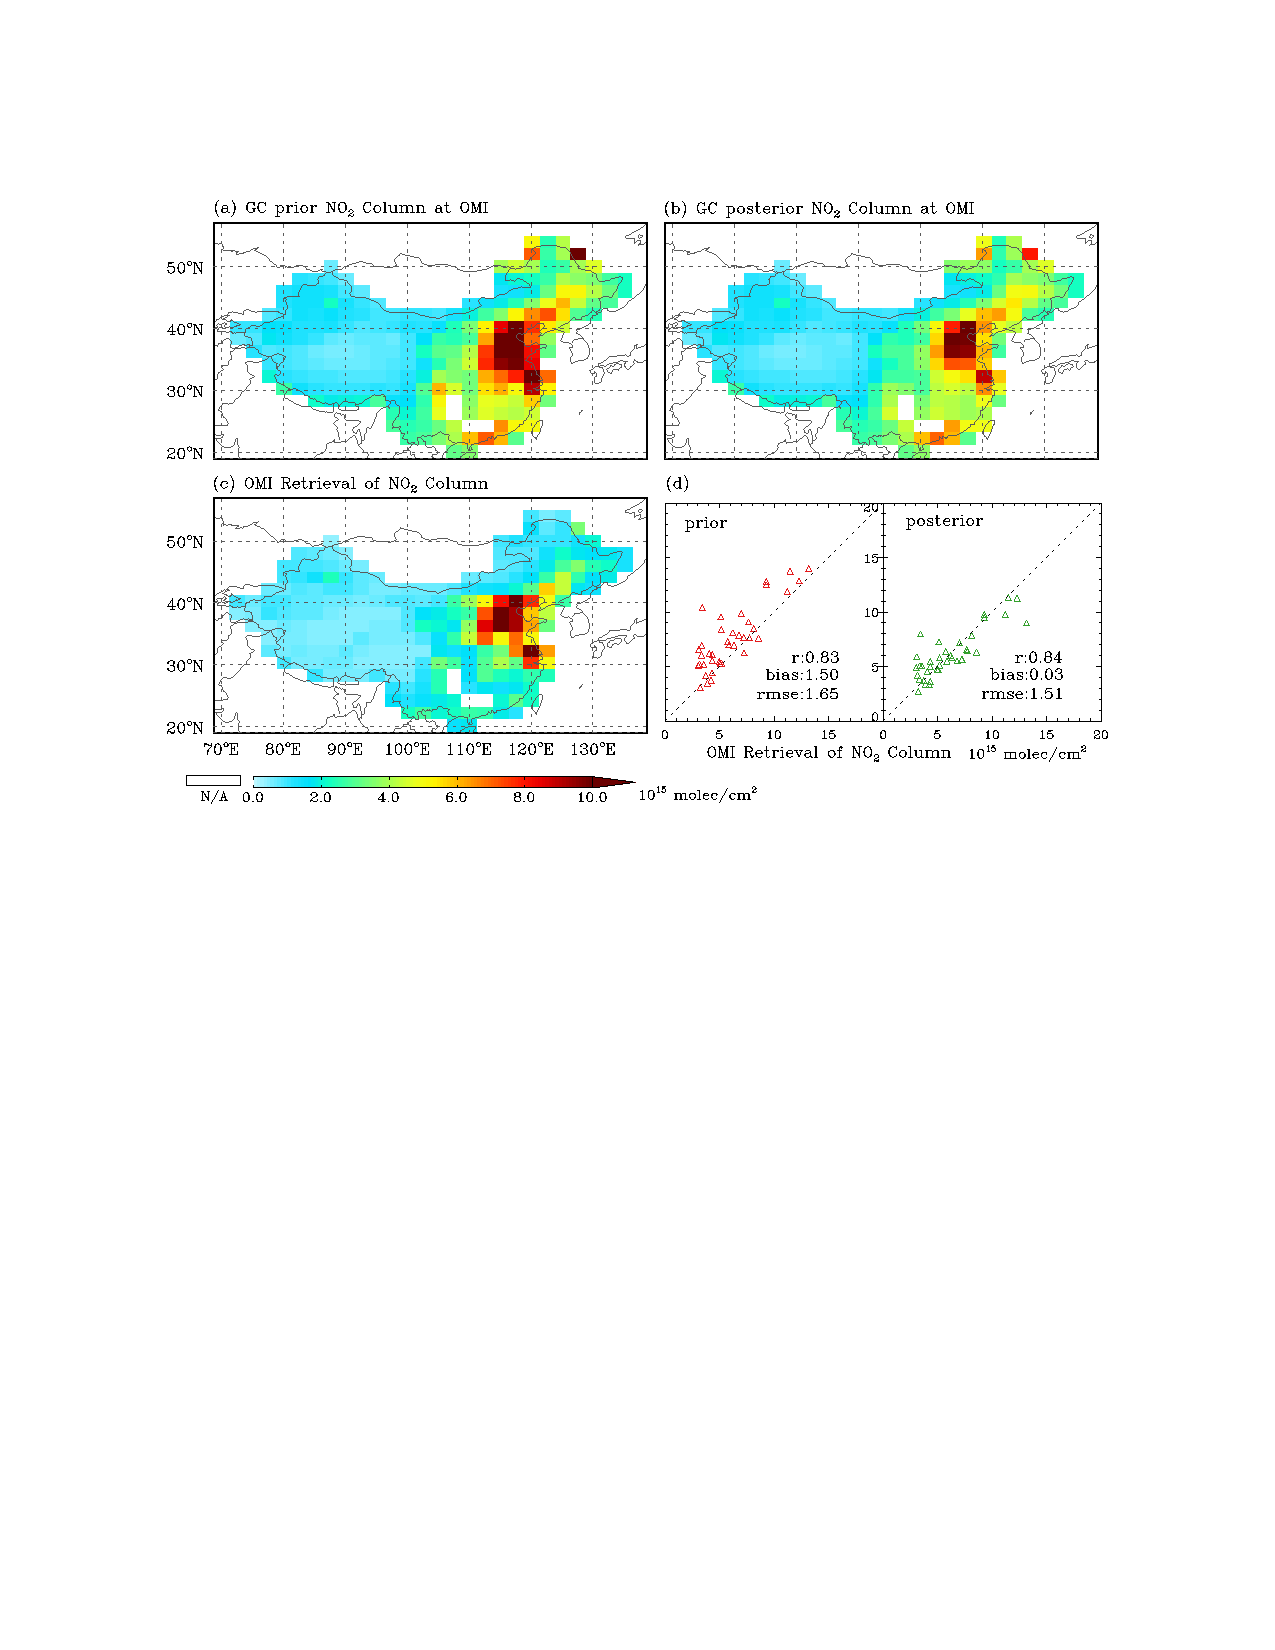
\includegraphics[width={0.9\textwidth}]{figures/a9.pdf}
  \caption{Same figure \ref{fig:misr1} but for comparison of the GEOS-Chem \ce{NO2} simulation with OMI column \ce{NO2} retrievals for the period of April 2008.  The OMI tropospheric column \ce{NO2} from Level 2 daily products with 0.25$^{\circ}$ by 0.25$^{\circ}$ resolutions are aggregated into GEOS-Chem grid cells.}
  \label{fig:omno2}
 \end{figure}

 %% Validation against surface SNA
 \begin{figure}[h]
  \centering
  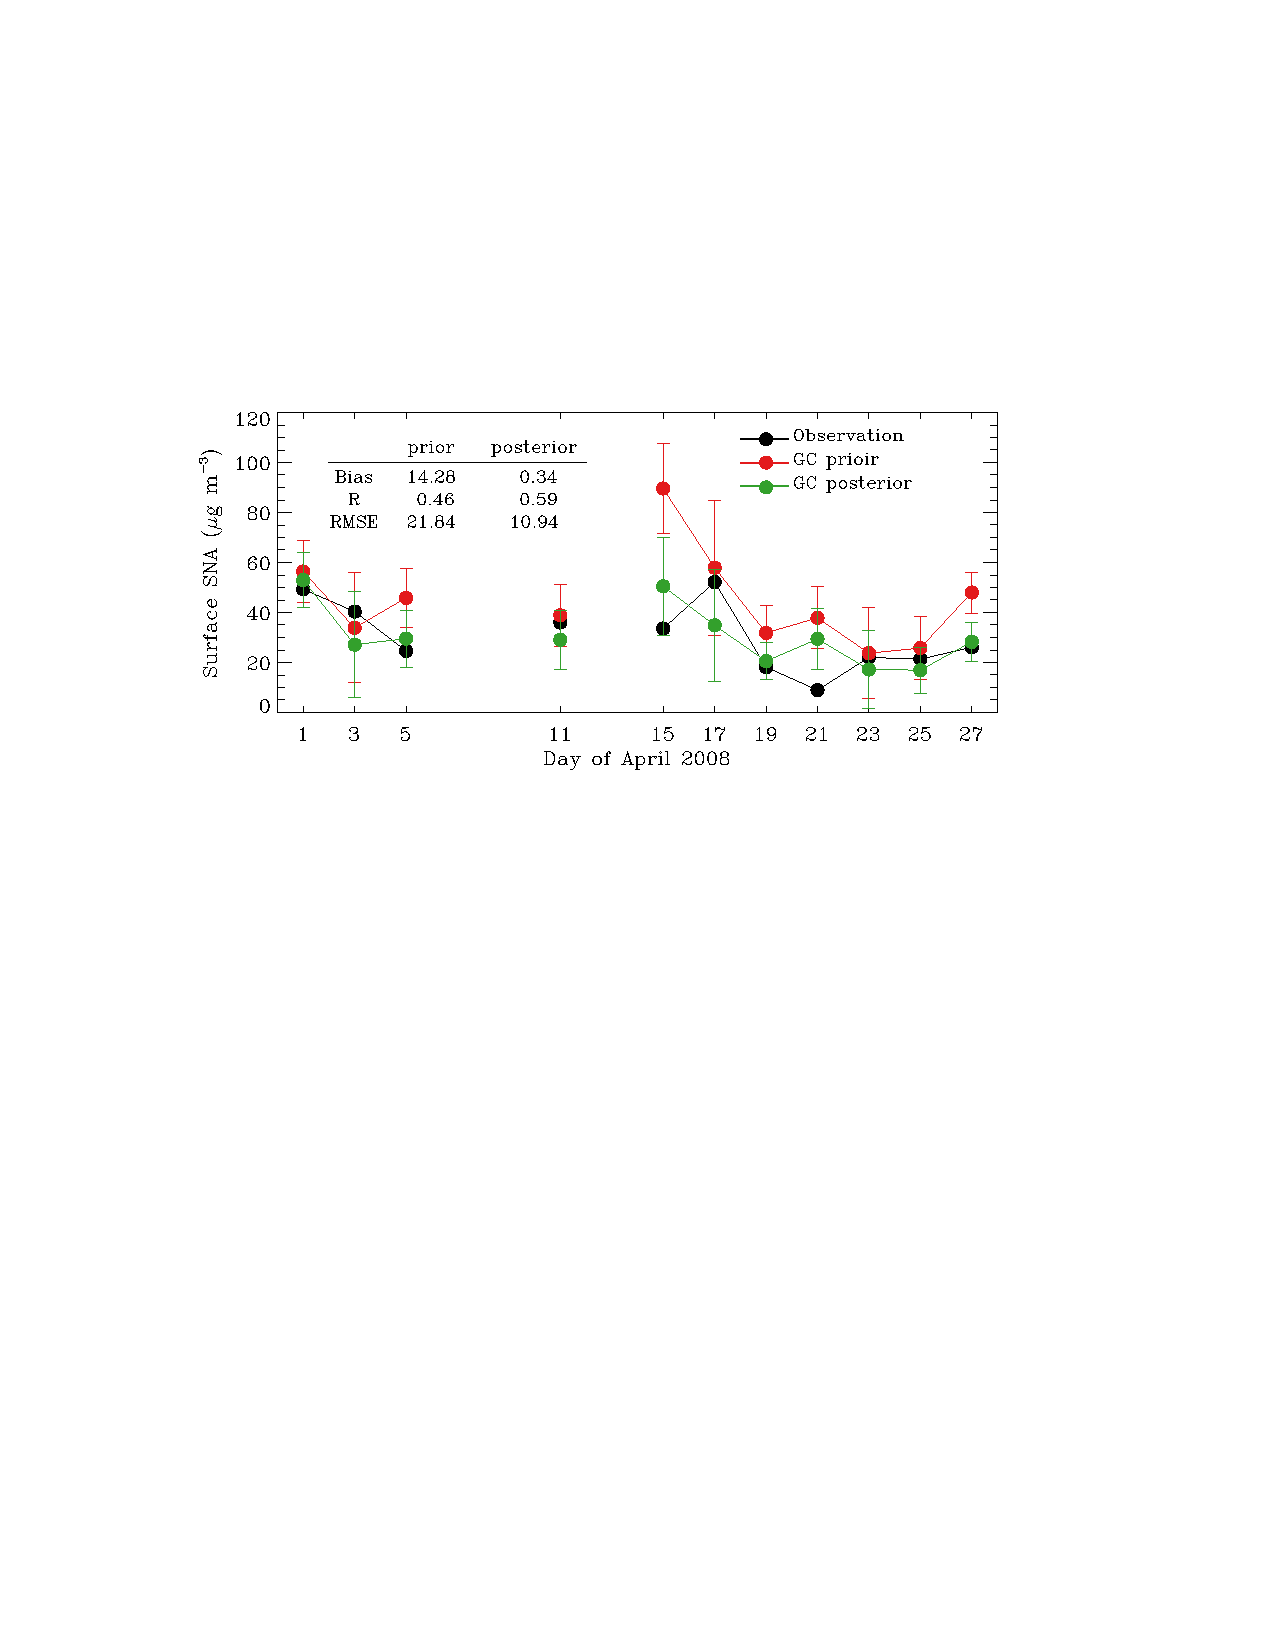
\includegraphics[width={0.8\textwidth}]{figures/a10.pdf}
  \caption{Comparison of the GEOS-Chem surface mass concentration of sulfate-nitrate-ammonium (SNA) aerosols with ground-based observations over Qingdao (120.34$^{\circ}$ E, 36.06$^{\circ}$ N), China. Discontinuity in time series is due to missing or quality filtered observations.}
  \label{fig:sna}
 \end{figure}

 %% Validation against surface PM10
 \begin{figure}[h]
  \centering
  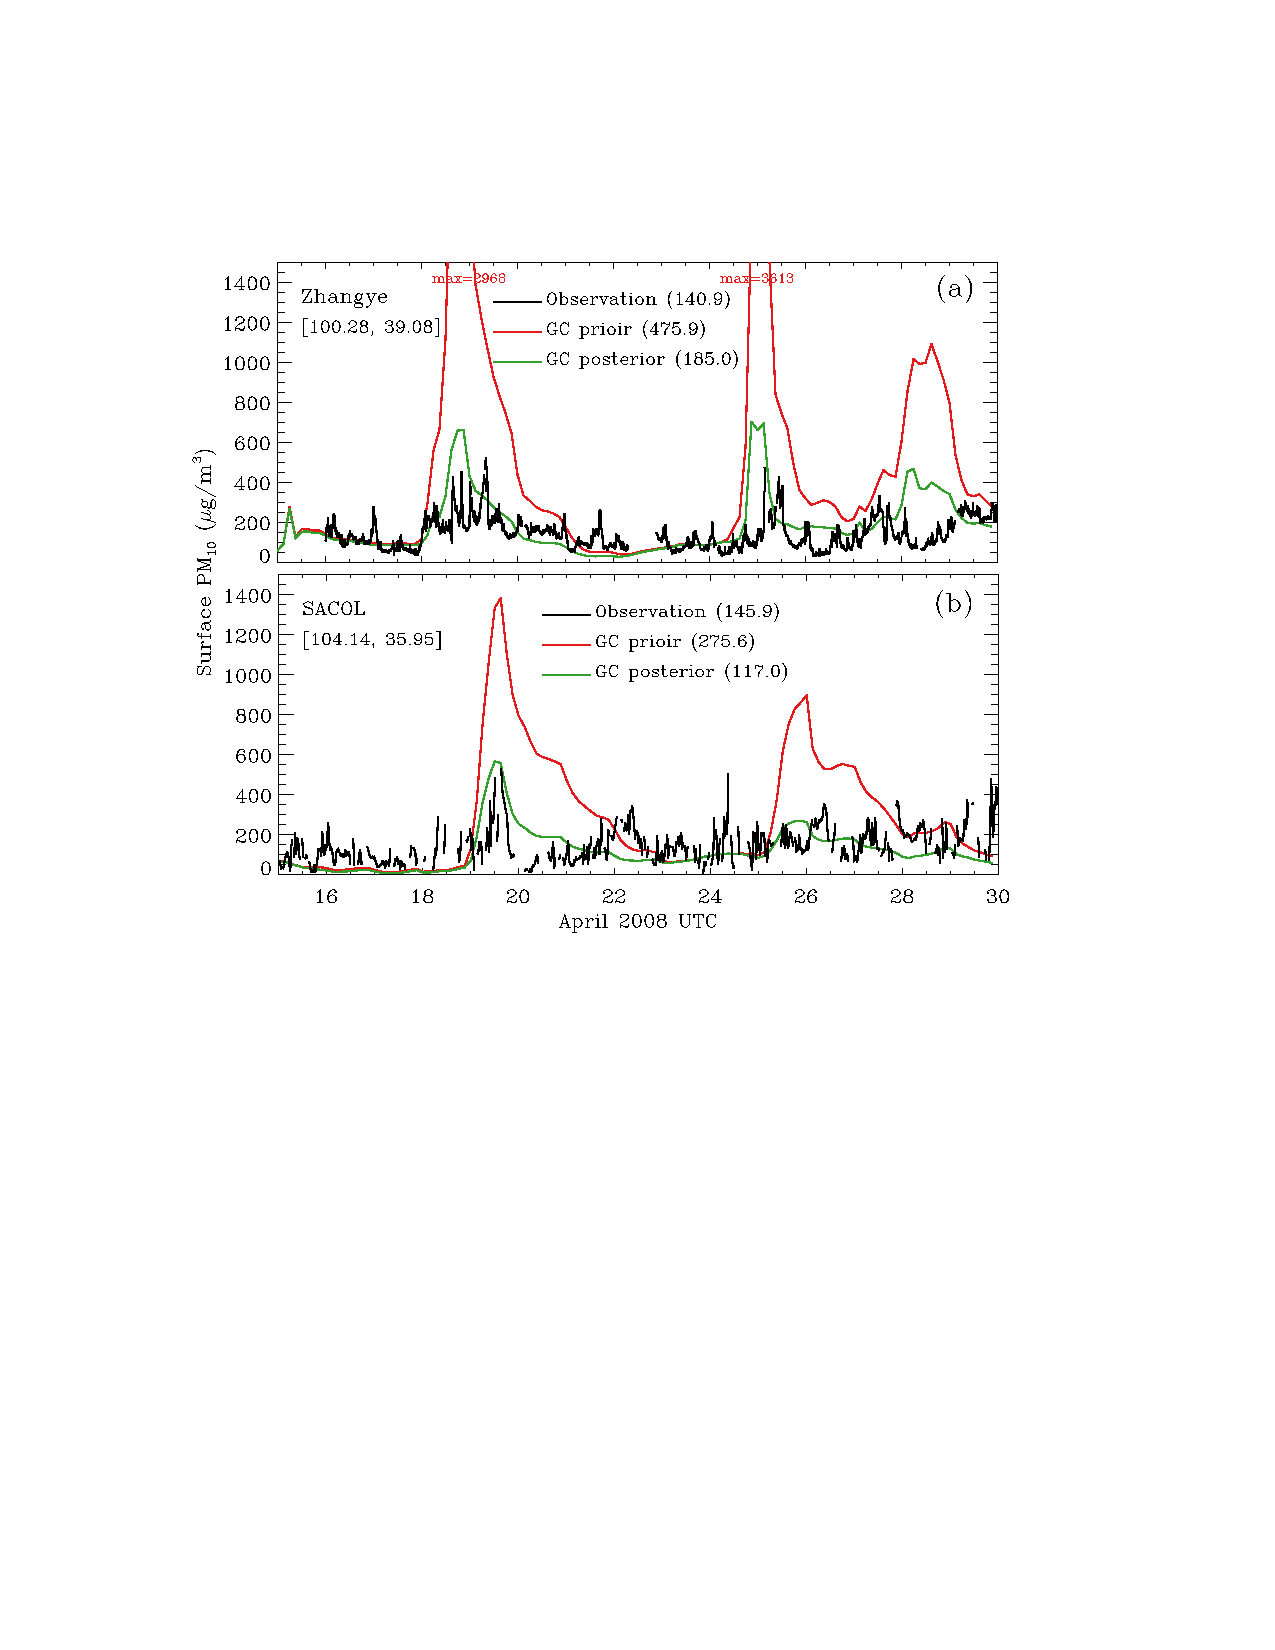
\includegraphics[width={0.95\textwidth}]{figures/a11.pdf}
  \caption{Time serial plot of the GEOS-Chem simulated surface PM\textsubscript{10} concentrations by prior (red) and posterior (red) aerosol emissions compared with the \textit{in situ} measured PM\textsubscript{10} (black) over Zhangye (a) and SACOL (b) stations for 15 – 30 April 2008; also shown are the average values over same the period. Discontinuity in time series is due to missing or quality filtered observations.}
  \label{fig:pm10}
 \end{figure}

 %% Validation Taylor diagram
 \begin{figure}[h]
  \centering
  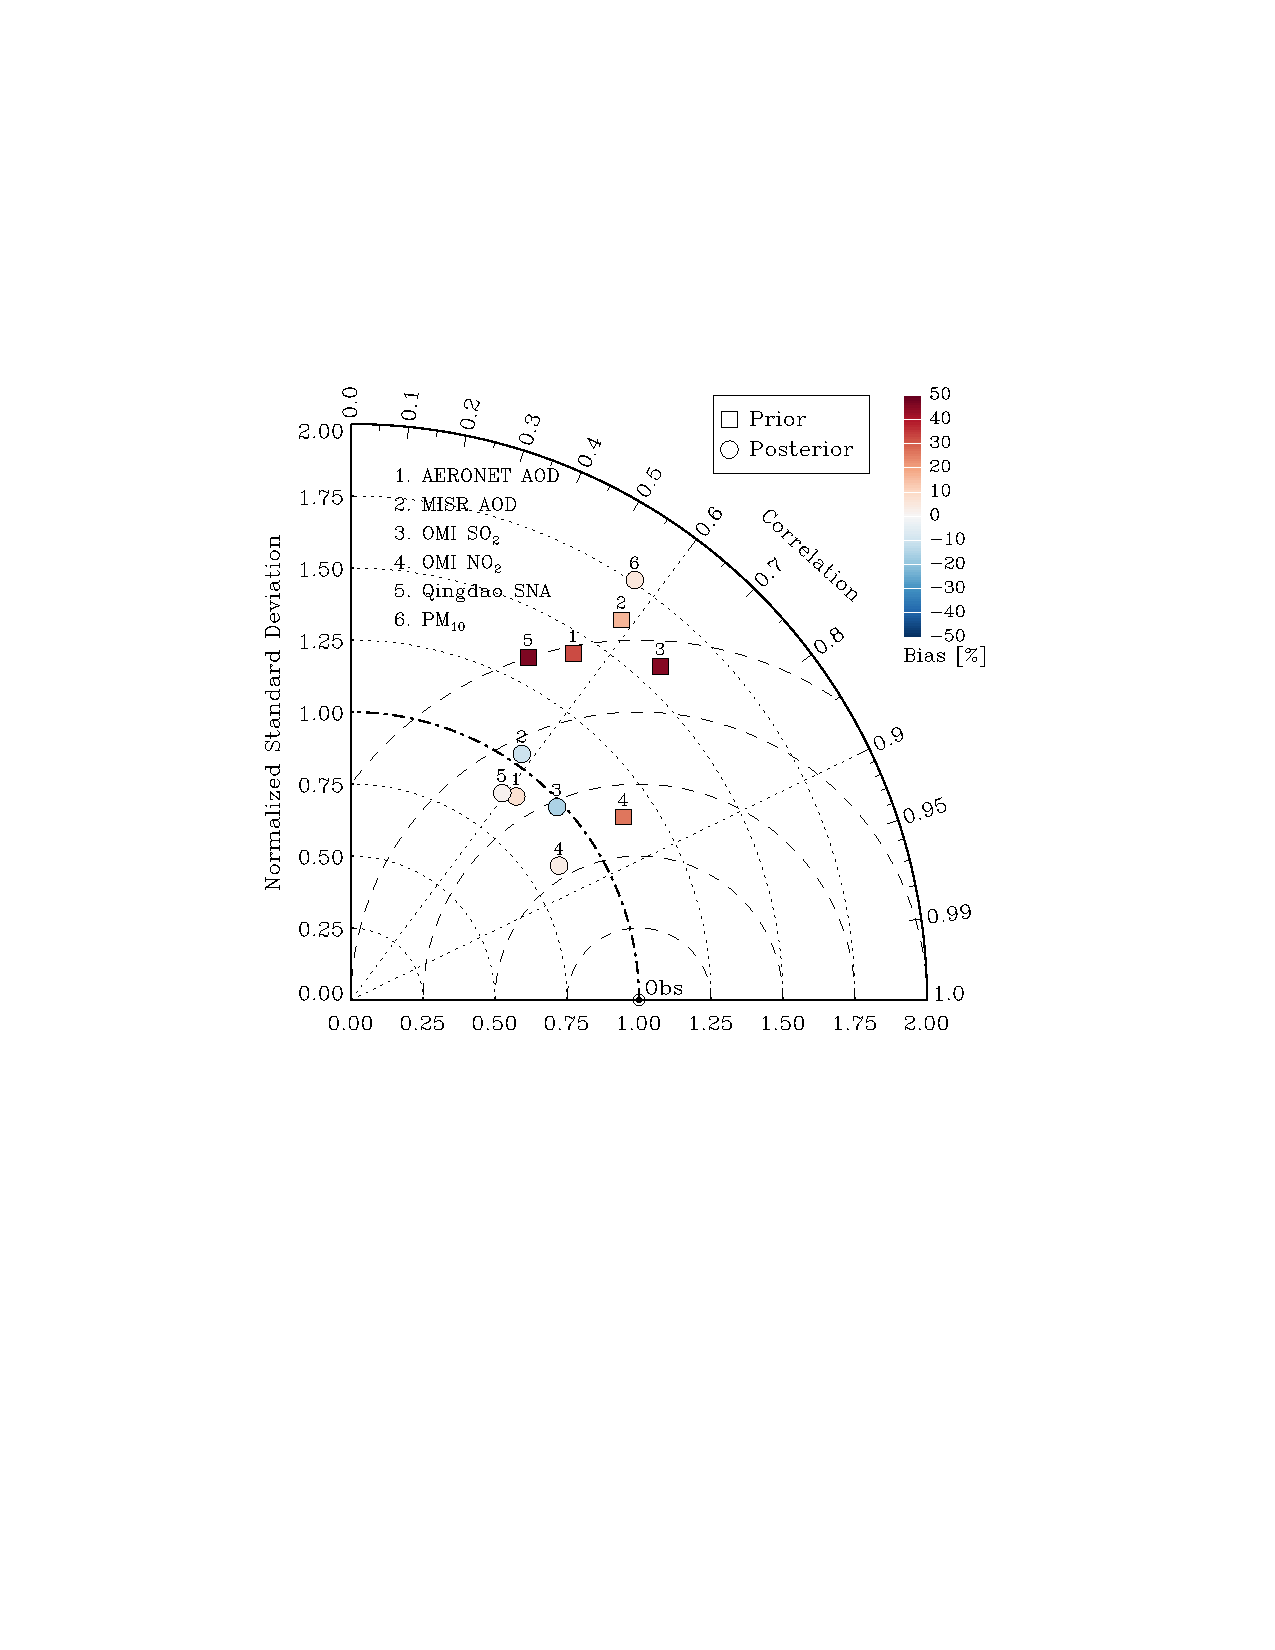
\includegraphics[width={0.66\textwidth}]{figures/a12.pdf} 
  \caption{Taylor diagram for the model evaluations before (squares) and after (circles) optimization when comparing against (1) AERONET AOD at 0.55 $\mu$m, (2) MISR 0.55 $\mu$m AOD, (3) OMI column \ce{SO2}, (4) OMI column \ce{NO2}, (5) surface SNA concentrations at Qingdao site, and (6) surface PM\textsubscript{10} concentrations measured at Zhangye and SACOL sites. The color coded on each point indicates the relative bias. It should be noted that the ratio of standard deviations and correlation coefficient between prior GEOS-Chem simulated and measured surface PM\textsubscript{10} over Zhangye and SACOL are 6.5 and 0.45, which makes the point number 6 for the prior simulation far beyond the range of this Taylor diagram. }
  \label{fig:taylor}
 \end{figure}


 %% Satellite AOD changes
 \begin{figure}[h]
  \centering
  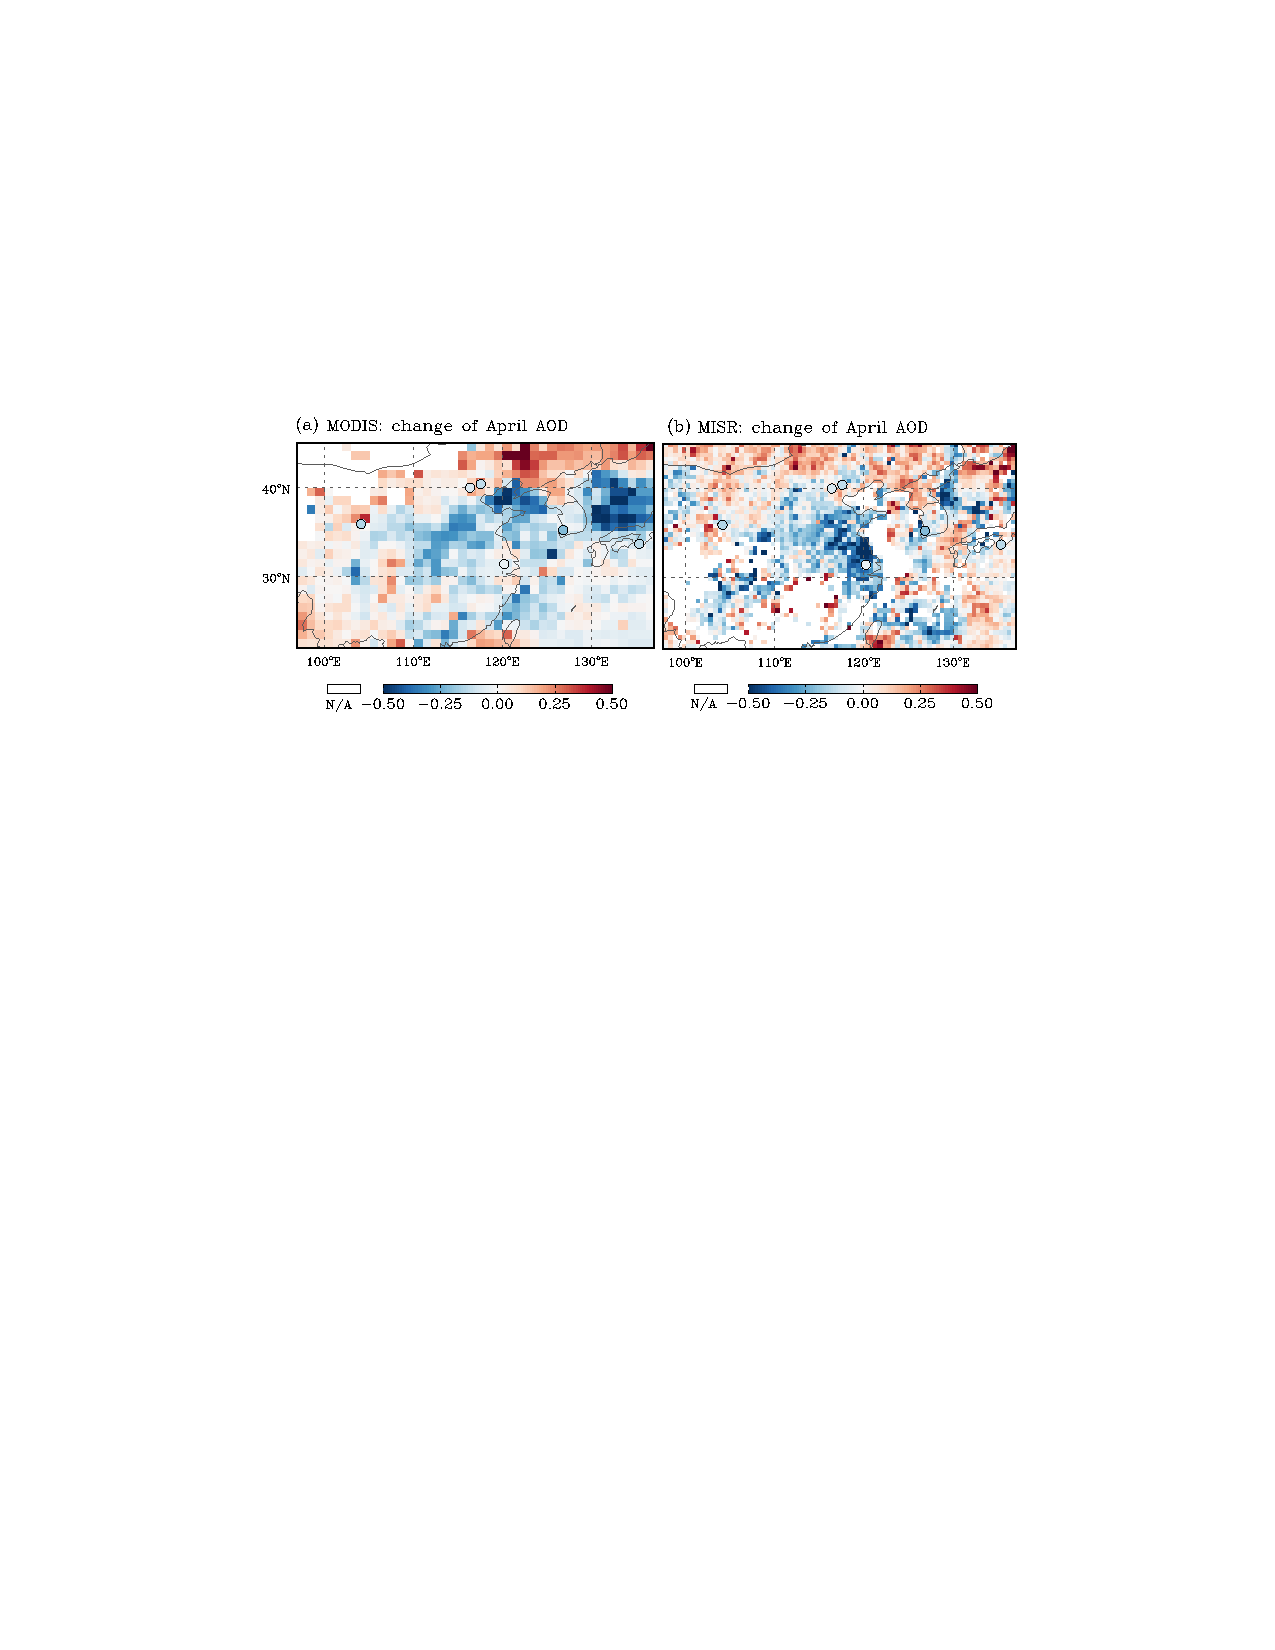
\includegraphics[width={0.85\textwidth}]{figures/a13.pdf}
  \caption{Change of April monthly 0.55 $\mu$m AOD from 2006 to 2008 from MODIS (a) and MISR (b) Level 3 daily products.}
  \label{fig:aodchange}
 \end{figure}

\section{Implications of Results}

\section{Summary}
